\scanpage{71}
% Reversed type shows through from the other face.
\[
\deleted{\unsure{R}}\ i_*{\unsure{G|\mathcal G}}^{\unsure{d}}(\unsure{k|F})
\]
\[
H^*(G)\Longleftarrow E_2^{pq}=H^p(X,R^qi_*(G))
\]

\figure{\begin{tikzpicture}[x=.72cm,y=.74cm]
\draw (-1.25,0)--(9,0); \draw (0,-.4)--(.09,5.1);
\draw (.07,4.7)--(4.05,0);
\foreach \x in {0,.8,1.75,2.55,4.05,4.9,5.9,7,7.8}{\draw (\x-.08,-.11)--(\x+.08,.11) (\x-.09,.1)--(\x+.08,-.09);}
\draw (3.16,-.13)--(3.32,.13);
\foreach \y in {2.66,3.58,4.7}{\draw (.04,\y) circle (.075); \draw (-.04,\y-.10)--(.15,\y+.12);}
\foreach \x/\y in {2.94/1.30,3.44/.73}{\draw (\x-.06,\y-.10)--(\x+.07,\y+.10) (\x-.07,\y+.1)--(\x+.07,\y-.1);}
\node[below] at (4.03,-.08){$n-1$}; \node[below] at (4.91,-.09){$n$}; \node[below] at (5.92,-.1){$n+1$};
\end{tikzpicture}}
\[
x\in\operatorname{Supp}R^qi_*(G)
\]
\[
\deleted{\operatorname{cd}(\bar x)+\varphi(x)}
\]
\[
\deleted{\unsure{\varphi}}\quad \operatorname{cd}(\bar x)+q\leq
\]

\figure{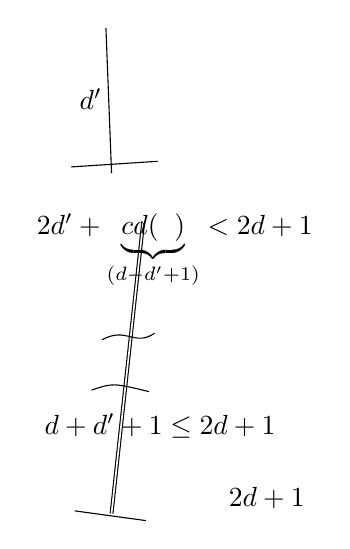
\begin{tikzpicture}[x=.65cm,y=.65cm]
\draw (0,-.18)--(-.11,2.65); \draw (-.79,-.06)--(.9,.05);
\node[left] at (0,1.26){$d'$};
\draw[double] (0,-6.83)--(.62,-1.12); \draw (-.72,-6.78)--(.67,-6.97);
\draw (-.39,-4.42)..controls (.03,-4.28)..(.73,-4.45);
\draw (-.19,-3.44)..controls (.29,-3.17) and (.44,-3.58)..(.84,-3.31);
\node[anchor=west] at (-1.65,-1.70){$2d'+\underbrace{\operatorname{cd}(\phantom{x})}_{(d-d'+1)}<2d+1$};
\node[anchor=west] at (-1.5,-5.12){$d+d'+1\leq 2d+1$};
\node[right] at (2.1,-6.52){$2d+1$};
\end{tikzpicture}}
\margin{$\deleted{\unsure{2d}}\ \leq d+1$ \unsure{?}\quad $1+2d'+(d-d'\deleted{\unsure{+1|2(d-1)}})=d+d'+1\leq 2d<2d+1$}

\[
\underline O_{X,\bar y}\otimes_X k(x)
\]
\[
\deleted{H^{\unsure{n|*}}(G)\mathbin{\unsure{-|\to}}H^{\unsure{n|*}}(\,}
\]
\[
\bullet\longrightarrow H^{n+1}(X)\longrightarrow H^{n+1}(G)
\]
\[
\deleted{q\leq\operatorname{cd}\underline O_{X,\bar y}\otimes}
\]
\[
q\leq\operatorname{cd}_p\operatorname{Frac}\underline O_{X,\bar y}
\]
\[
\underbrace{\operatorname{cd}(\bar y)}+q\,\underbrace{\operatorname{cd}_p\operatorname{Frac}\underline O_{X,\bar y}}<n\qquad y\in\bar x
\]
\[
\deleted{\varphi(y)<\varphi(x)-\operatorname{cd}_{\ell}(\,}
\]

\uline{Lemme}.
\[
\boxed{\begin{aligned}
&\operatorname{cd}_{\ell}(k(x))\leq n\\
&\forall Y\ \text{\unsure{vrai|rem|réunion} de } X,\quad \operatorname{cd}_{\ell}(Y)<n\\
&\forall y\in X,\ y\ne x,\quad \operatorname{cd}_{\ell}(\bar y)+\operatorname{cd}_{\ell}\operatorname{Frac}\underline O_{X,\bar y}<n
\end{aligned}}\ \overset{\displaystyle\operatorname{cd}_{\ell}(X)\leq n}{\nearrow}
\]
\[
2\dim\bar y+\underbrace{\dim\underline O_{X,\bar y}}_{\unsure{\in|\leq|\oplus}\dim\text{“}X-\dim\bar y}\qquad
\begin{aligned}\dim X+\dim\bar y&<\\&2\dim X\end{aligned}
\]
% archive sheet number: 70
